\section{Problem Setting}
\label{sec:problem}

\begin{figure*}[t]
\centering
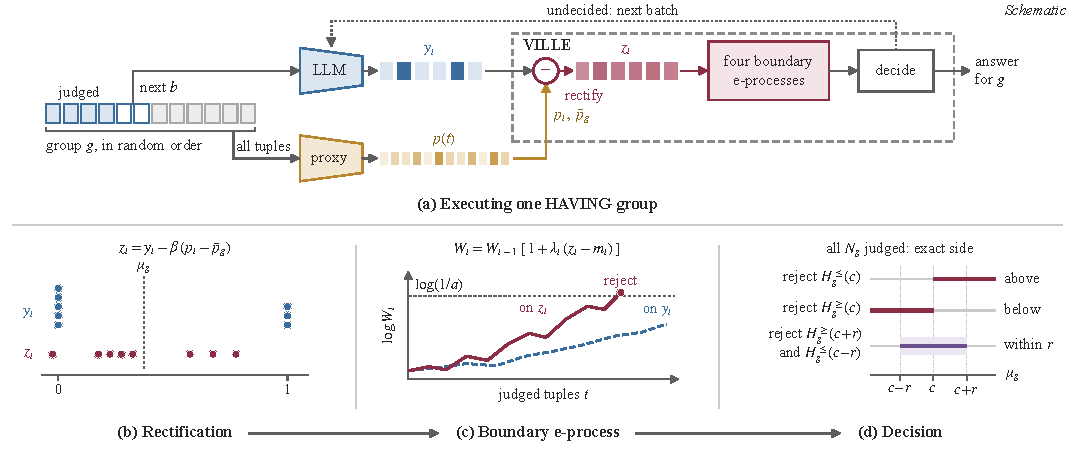
\includegraphics[width=\textwidth]{figures/overview_mechanism.pdf}
\caption{\sys{} executing one HAVING group. (a) In one random order, the LLM judges the next $b$ tuples, the proxy scores all tuples once, and \sys{} rectifies the judgments and updates four boundary e-processes until a decision is certified. (b) Rectification keeps the group mean $\mu_g$ for any proxy, and an informative proxy pulls 0/1 judgments toward it (eight tuples, $\beta=1$). (c) Each e-process bets against the remaining-population null mean $m_t$ (\Cref{eq:mt}) and rejects at wealth $1/a$, $a=\alpha/(2K)$; betting on $y_t$ (dashed) is slower. (d) Rejections that certify each answer; an exhausted group is decided exactly.}
\label{fig:overview}
\end{figure*}


\subsection{Decision queries over an expensive attribute}

We consider a relation $R$ whose tuples are partitioned into $K$ groups by a grouping key, for example the product, brand, category, or year of a review.
Group $g$ contains $N_g$ tuples.
The sizes $N_g$ are known, because counting tuples per group only reads the grouping column.
Each tuple $t$ has an \emph{expensive attribute} $y(t)\in[y_{\min},y_{\max}]$ that is obtained by one call to a large language model (LLM).
For a semantic predicate such as ``does this review report a defective product?'', $y(t)\in\{0,1\}$.
For a semantic score such as ``how positive is this review, from 1 to 5?'', $y(t)\in[1,5]$.
We treat the LLM as a deterministic function of the tuple, as with greedy decoding and a cache, so each tuple is judged at most once.
The query targets the group means
\begin{equation}
\mu_g=\frac{1}{N_g}\sum_{t\in g} y(t), \qquad g=1,\dots,K .
\end{equation}
\texttt{AVG} over a score and the fraction of tuples satisfying a predicate are both of this form.
\texttt{COUNT} and \texttt{SUM} equal $N_g\mu_g$, so decisions on them reduce to decisions on $\mu_g$ with a rescaled threshold.

The system also has a \emph{proxy} $p(t)\in[y_{\min},y_{\max}]$ for every tuple, for example a small classifier on n-grams or embeddings.
Proxies are orders of magnitude cheaper than LLM calls and are routinely used to optimize queries with expensive model predicates~\cite{blazeit,supg,abae,lotus,bargain}.
We make no assumption on proxy quality: a poor proxy may cost efficiency, but it must never cost correctness.

We study three \emph{decision queries}, whose answers are discrete:
\begin{itemize}
\item \textbf{HAVING}: return the groups with $\mu_g>c$ for a threshold $c$.
\item \textbf{ORDER BY}: return the groups ranked by $\mu_g$.
\item \textbf{Top-$k$}: return the $k$ groups with the largest $\mu_g$ (\texttt{ORDER BY \dots\ LIMIT} $k$).
\end{itemize}
These queries are the backbone of dashboards and of LLM-generated reports (``which product lines have more than 20\% defect complaints?'', ``rank the stores by service quality'', ``the five categories with the most negative reviews'').
They are also the queries that a sampling-based answer can get \emph{wrong}: an estimate that is off by one percentage point is harmless, whereas a swapped pair in a ranking or a group on the wrong side of a threshold is a wrong answer.

\subsection{Correctness with an indifference margin}

Exact decisions cannot be certified from samples when two means coincide or a mean sits on the threshold.
We therefore adopt an indifference margin $r>0$, a standard device in sequential selection~\cite{bechhofer1954,lucb}.

\begin{definition}[$r$-correct answers]
\label{def:rcorrect}
A HAVING answer $A\subseteq[K]$ is $r$-correct if every group with $\mu_g\ge c+r$ is in $A$ and no group with $\mu_g\le c-r$ is in $A$.
A ranking is $r$-correct if group $i$ precedes group $j$ whenever $\mu_i\ge \mu_j+r$.
A Top-$k$ answer $S$ with $|S|=k$ is $r$-correct if $\min_{i\in S}\mu_i\ge \mu_{(k)}-r$, where $\mu_{(k)}$ is the $k$-th largest group mean.
\end{definition}

Groups or pairs inside the margin may be reported either way.
The margin is part of the query, for example $r=5\%$ of the overall mean.
It permits early termination near a boundary through an ``indifferent'' certificate. Every finite group also has an exact fallback when all its tuples have been judged.

\subsection{Certified answers and cost}

A system answers a decision query by repeatedly sending batches of sampled tuples to the LLM, updating its statistics, and deciding when to stop.
Analysts and LLM agents also inspect intermediate answers and stop when the answer looks stable.
Both behaviours are forms of \emph{continuous monitoring}.
A fixed-sample confidence interval does not survive them: its coverage holds only at one pre-specified sample size~\cite{ramdas2023savi,johari2022}.

\begin{definition}[Certified decision query]
\label{def:certified}
An algorithm certifies a decision query at level $\alpha$ if, for every data instance, every proxy, and every (possibly data-dependent) stopping time, the probability that it reports an answer that is not $r$-correct is at most $\alpha$.
\end{definition}

The cost of an algorithm is the number of LLM calls it issues, $C=\sum_g n_g$, where $n_g\le N_g$ is the number of tuples of group $g$ that were judged.
We report $C/\sum_g N_g$, the fraction of the full evaluation that was needed.
Proxy scores are computed once for all tuples and their cost is amortized; we report it separately.
The goal is to certify every decision query at level $\alpha$ with as few LLM calls as possible.
